\section{Motor Thrust Testing}\label{appendix_thrust}
The 4th semester project in mechatronics is based on building a VTOL drone. For the drone to take flight, 
sufficient thrust provided by the propellers attached to the motors of the drone is required. Thus,
the following is the report of thrust testing using different motors and propellers.
Initial testing setup

\subsection{Initial Assumptions}
The initial idea to test the thrust provided by a certain motor was to create a x-shaped frame where, 
the motors were connected to their respective corners and a bolt was tightened in the centre as a means of weight. 
The frame with the motors were then placed on a scale where the motors were facing in the direction of the ceiling, 
thus meaning that propellers were pushing the air downwards and the setup upwards. The initial weight of the frame was then noted, 
where after powering up the motors, the weight of the setup would decrease due to the thrust. 

\subsection{Initial Results}
The setup of the bolt supporting the frame on the scale was unstable, and because of that the wiring of the motors had also
interfered with the weight. Additionally, as the propellers were pushing the frame with a certain thrust force, 
the air that was being pushed down also had the same force. Therefore, as the frame was very close to the scale, 
the force by which the setup was being lifted by was also being pushed down by the air on the scale, thus making almost no 
changes on the scale readings. 

\begin{figure}
    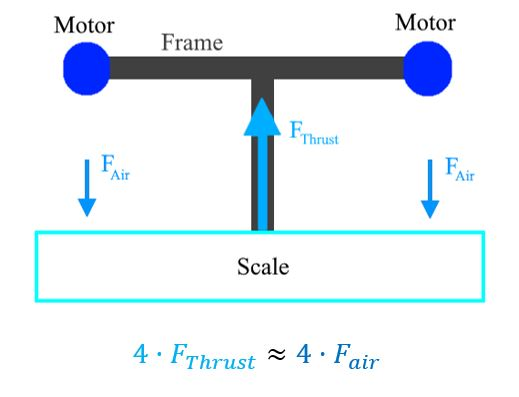
\includegraphics[width=\linewidth]{pictures/control/Motor thrust 1.jpg}
    \caption{Initial Thrust Setup}
    \label{fig:Initial Thrust Setup}

\end{figure}

\subsubsection{Final Assumptions}
To fix the problems of the initial test setup, a second version of the x-shaped frame was made where the corners were connected to 3d printed pillars, 
to make the system more stable. Additionally, instead of placing all the motors at each corner and measuring thrust, only one motor would be placed in the centre instead, 
as the other motors were identical and thus would produce close to identical thrust. Moreover, the motors would now be placed in a direction opposite to the ceiling as then the air would not be pushed on the scale, 
but the frame would be. Thus, the additional weight that occurs after the motors are powered on would be equal to the thrust provided by the motor and propeller.

\begin{figure}
    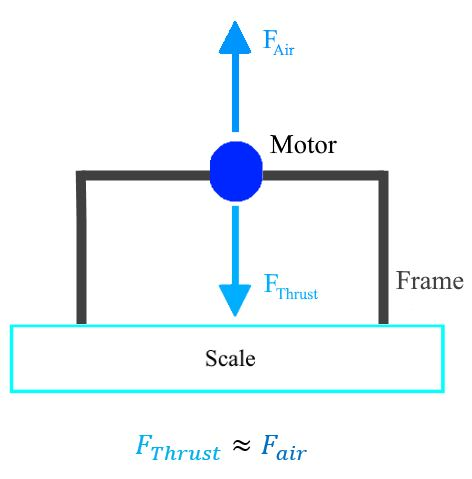
\includegraphics[width=\linewidth]{pictures/control/Motor thrust 2.jpg}
    \caption{Final Thrust Setup}
    \label{fig:Final Thrust Setup}

\end{figure}

\subsubsection{Final Results}

The motor used had an operating voltage window of 0-4,2 volts, therefore the motor was tested between 1-4,2 volts incremented with 0,1 volts. 
Characterizing the motor yielded the following results:

\begin{figure}
    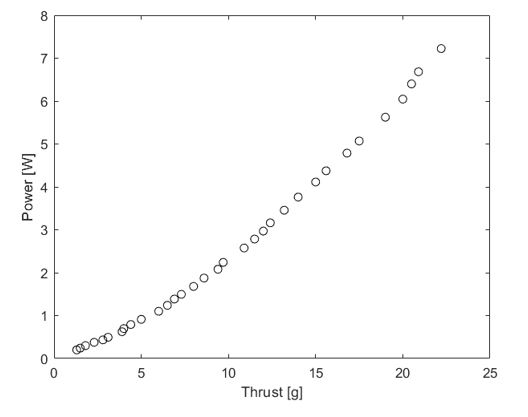
\includegraphics[width=\linewidth]{pictures/control/Graph Thrust.jpg}
    \caption{Final Thrust Setup}
    \label{fig:Final Thrust Setup}

\end{figure}

It became clear that the total thrust that could be produced by a single motor was 17.5 grams at 3.7 Volts 
(The minimum level of the battery). Subtracting the weight of the motor itself, the motor can produce a net thrust of 12.4 grams, 
and since the drone would be flown in a quad configuration, the total net thrust possible for the four motors were 49.6 grams at lowest voltage. 
This then set the limits of how heavy the drone could be, and since a general rule of thumb is that the motors need to produce double the needed thrust to lift the drone , 
it’s clear that the remaining components of the drone can weigh 24,8 grams for it to handle optimally. At maximum voltage level of the battery, a motor produces 22.2 grams of thrust, 
so an excess of 17,1 grams subtracting the motors weight itself. So at maximum voltage level, the drones remaining components can weigh 34.2 grams.  
